\documentclass{article} 
	\usepackage{fontspec,booktabs,xunicode,xltxtra,amsmath,amssymb,caption,colortbl,float,caption,algorithm,algpseudocode}
	\usepackage{graphicx}
	\usepackage{pgfplots}
	\usepackage{xeCJK}
	\setCJKmainfont{MSYH.ttc}
	\title{人工智能基础\\最佳split点的寻找}
	\author{孔静-2014K8009929022}

\begin{document}   
	\maketitle
	\section{问题}\
	
		“Introduction to Boosted Trees”这个slides的39页上的问题,
		
		提交伪代码,并分析时间复杂度
		
		\begin{figure}[htp]
			\centering
			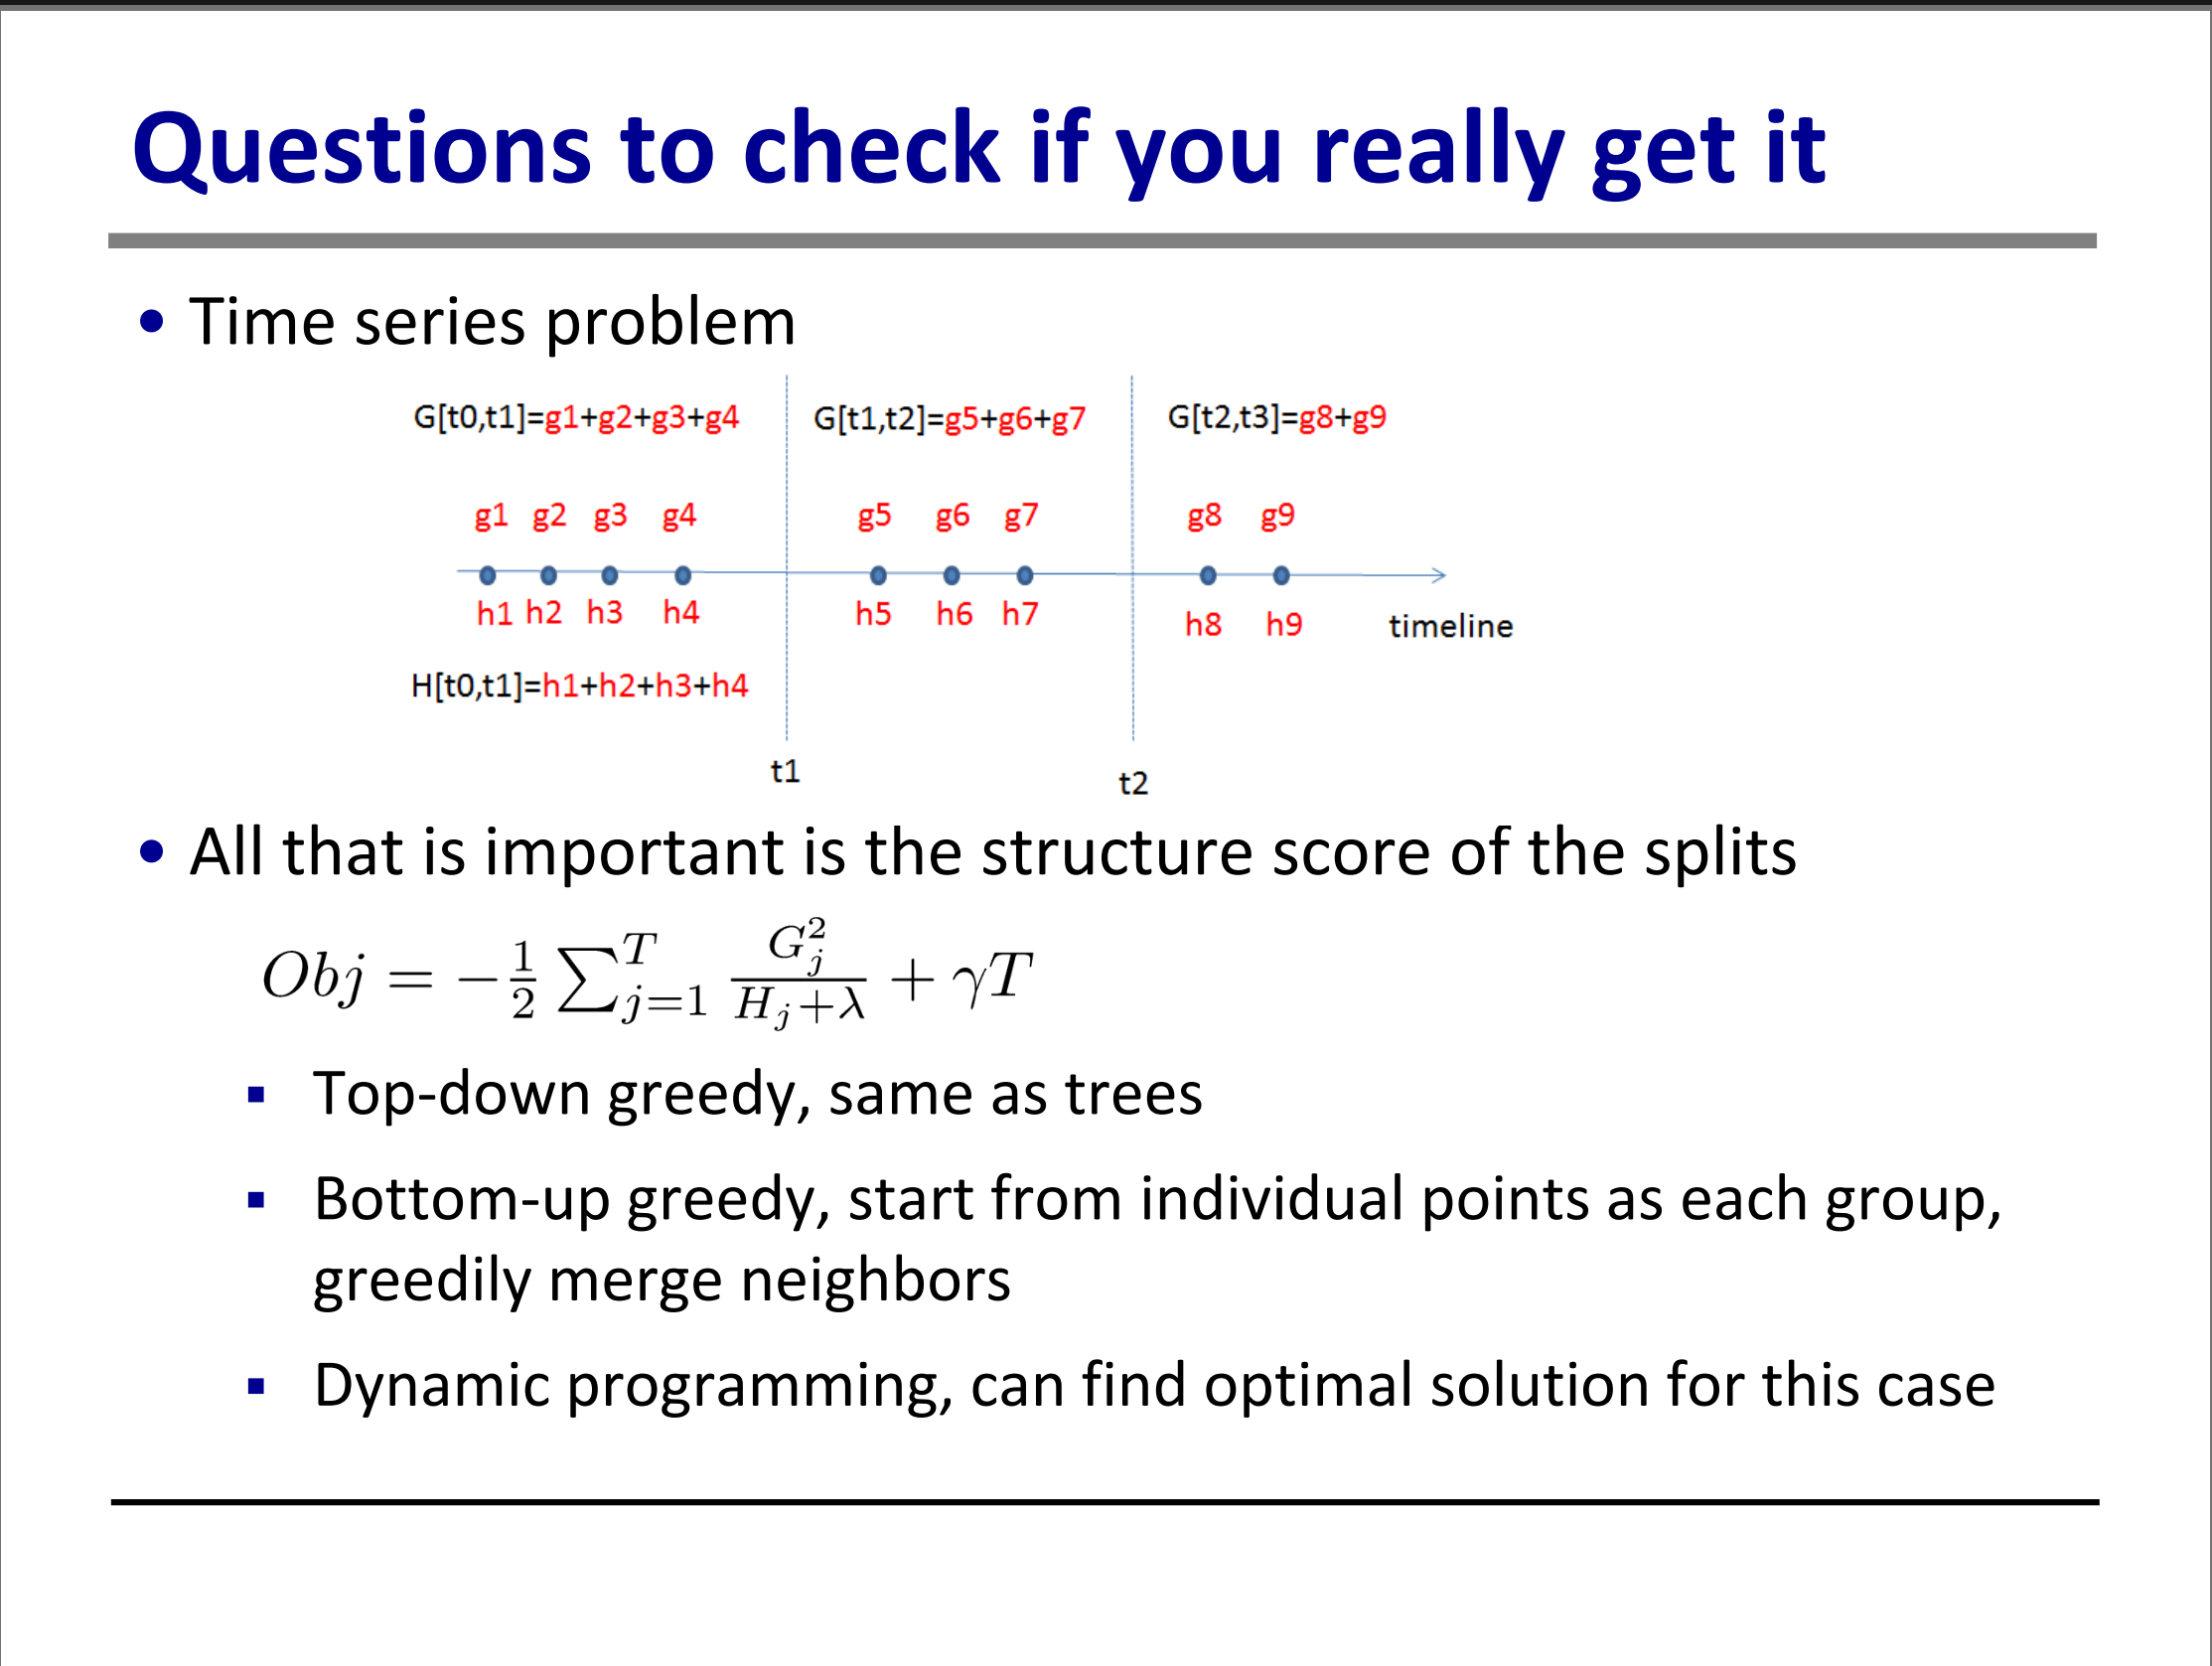
\includegraphics[width=12cm]{picture}
			\label{Introduction to Boosted Trees-p39}
		\end{figure}
	
		ORZ,写完以后想起来要用动态规划写,但好像我用的是分治>.<。但讲道理差别不大嘛,动态规划用上一次的东西往下传,在这个题里面,分治也可以把这个信息往下传嘛!差别不是很大嘛!懒得改了=.=
	\newpage
	\section{伪码}
		\begin{algorithm}[H]
			\caption{Find The Split}
			\begin{algorithmic}
				\Procedure {Main}{g,h,n,a}
				\State k = 1
				\State FindSplit(g,h,n,a)
				\State \textbf{return} $Split$ 
				\EndProcedure				
			\end{algorithmic}
			\begin{algorithmic}				\Procedure {GetScore}{G,H,T}
				\State $O{\rm{bj =  - }}\frac{1}{2}\sum\nolimits_{\rm{j}} {\frac{{G{{[j]}^2}}}{{H{\rm{[j] + }}\lambda }}} {\rm{ + 3}}\gamma$
				\State \textbf{return} $Obj$ \Comment 计算分数 
				\EndProcedure				
			\end{algorithmic}
			\begin{algorithmic}
				\Procedure {GetGain}{GL,GR,HL,HR}
				\State $Gain = \frac{1}{2}[\frac{{G{L^2}}}{{HL + \lambda }} + \frac{{G{R^2}}}{{HR + \lambda }} - \frac{{{{(GL + GR)}^2}}}{{(HL + HR) + \lambda }}] - \gamma$
				\State \textbf{return} $Gain$ \Comment 计算增益 
				\EndProcedure				
			\end{algorithmic}
			\begin{algorithmic}
				\Procedure {FindSplit}{g,h,n,a} \Comment g,h为n个梯度数据,a为增益阈值
				\State $G[1] = \sum {g[i]}$
				\State $h[1] = \sum {h[i]}$
				\State Obj[0] = GetScore(G, H, 1) \Comment 用0位存储不分割的分数
				\State Split[0] = 0 \Comment 用0位存储分割点,0是不分割
				\State Gain[0] = a \Comment 用0位暂时存储比较值,a是阈值
				\For{i = 1 to n}
				\State $GR = \sum\nolimits_{j = 1}^i {g[j]}$
				\State $GR = \sum\nolimits_{j = i + 1}^n {g[j]}$
				\State $HL = \sum\nolimits_{j = 1}^i {h[j]}$
				\State $HR = \sum\nolimits_{j = i + 1}^n {h[j]}$
				\State Gain[i] = GetGain(GL, GR, HL, HR)
				\If {Gain[i] > Gain[0]} \Comment 贪心,找出最大的增益
				\State Gain[0] = Gain[i]
				\State Split[0] = i
				\EndIf
				\EndFor
				\algstore{brbreak}
			\end{algorithmic}
		\end{algorithm}
		\begin{algorithm}[H]
			\caption{Find The Split}
			\begin{algorithmic}
				\algrestore{brbreak}
				\If { Split != 0 } \Comment 如果找到了分割点,保存数据,分治继续寻找
				\State Obj[k] = Obj[k-1] - Gain[0]
				\State Split[k] = Split[0]
				\State k = k + 1 
				\For {i = 1 to Split}
				\State gl[i] = g[i]
				\State hl[i] = h[i]
				\EndFor
				\For {i = Split + 1 to n}
				\State gr[i - Split] = g[i]
				\State hr[i - Split] = h[i]
				\EndFor
				\State FindSplit(gl, hl, Split, a)
				\State FindSplit(gr, hr, n - Split, a)
				\EndIf
				\EndProcedure	
			\end{algorithmic}
		\end{algorithm}
	
	\section{分析}\
		
		单层贪心,遍历O(n);分治处理多层,O(logn)。
		
		综上,时间复杂度是O(nlogn)。
	
	\section{参考}\
		
		毕竟英文渣,看了网上翻译版的=.=
		
		http://www.52cs.org/?p=429
		
		http://blog.sina.com.cn/s/blog\_7103b28a0102w6qa.html
		
	\end{document}
\end{document}